\chapter{Background}
\label{chap:background}

\section{The Python Programming Language}
% A dynamic language; why calling missing API can only be reported until runtime

Python is dynamic programming language, the interpreter translates Python source code contained in a \textit{.py} file to Python byte code and stores it in a \textit{.pyc} file. And it executes many common programming behaviors such as program extension, code insertion, object and definition extension, and type system modification which static programming languages perform during compilation. Depending on the arguments passed into a Python interpreter, it can read and execute single lines of command or command blocks interactively when connected to a tty device's standard input, or it can execute all statements\footnote{Here "statement" and "command" are used interchangeably} in a Python source file at once when called when the input is a file.

As a \textit{strongly} typed programming language, data types of Python variables are tracked internally but cannot be implicitly changed by the interpreter to compromise for the successful execution of the current command. But as a \textit{dynamically} typed programming language, programmers have great freedom of explicitly changing the type of a variable by assigning it new values, and variable types cannot be checked or retrieved until runtime. Due to the lack of inspections during interpretation, errors such as invocations of undefined APIs and passing arguments of wrong data types often ruin the programming experience of Python.

\section{Python API Evolution}
% Briefly summarize Hengcheng and Zhaoxu's findings

There are 14 types of change patterns found in Python framework evolution, 5 of which are specific to Python frameworks in comparison to Java frameworks due to the language features of Python. Evolutions might induce crashes, including 10 types of runtime exceptions, or unexpected behaviors in client applications, more frequently than those in Java frameworks and Java client applications~\cite{DBLP:conf/wcre/ZhangZWTLX20}.

\subsection{Breaking and Non-breaking Changes}
% Distinguish between breaking/non-breaking changes

Based on their effects, API changes can be classified into \textit{breaking changes} and \textit{non-breaking changes}~\cite{api-evo-refactoring} (\hyperref[lst:break-nonbreak-change]{Listing 2.1}).

\begin{enumerate}
	\item \textbf{Breaking Changes} Among the observed Python framework evolution patterns, it is noticed that some changes are not backward-compatible and if client programs invoked obsolete APIs after updating dependent framework packages to newer versions that introduced those kinds of changes, they would suffer from compilation complaints or runtime problems. These changes that would lead to exceptions or unexpected behaviors are called \textit{breaking changes}.
	\item \textbf{Non-breaking Changes} Contrary to breaking changes, \textit{non-breaking changes} do not obstruct previously existing APIs, though could insert new APIs. Dependencies that have gone through non-breaking changes in updates would not cause any exceptions or unexpected behaviors in client programs.
\end{enumerate}

\begin{figure}[!t]
	\lstinputlisting[
		language=diff,
		caption={Breaking \& Non-breaking changes},
		label={lst:break-nonbreak-change}
	]{code_snippets/break_nonbreak_changes.diff}
	\vspace{-5mm}
\end{figure}

\subsection{Atomic and Compound Changes}
% Distinguish between atomic/compound changes

From the perspective of observing differences between two versions of an evolved source file, \textit{atomic changes} are insertion of new code and deletion of old code. This is different from the perspective of performing actions that produce those differences, in the case that an update action developer takes would be observed as a delete action and an insertion action in the aftermath, making it a \textit{compound change} in our definition. An empirical study on compound changes by our definition will be discussed in chapter \hyperref[chap:compound-changes]{Compound Changes}.

Automation of detecting such compound changes is an important goal this project aims to achieve, as previous tools did not deliver. And comprehending the intents of such changes would help provide better API evolution and usage messages to client software developers.

\section{Tree Differencing}

The tree-to-tree correction problem was first studied in~\cite{tree-edit-p},~\cite{tree-correction-p}. It is a high-dimensional generalization of the string-to-string correction problem, and aims to determine the minimum cost of edit operations required to transform one tree to another. Since a Python source program could be parsed into an AST, tree-differencing algorithms could be applied to unmask the actual changes underneath different library\footnote{Here "library" and "framework" are also used interchangeably} release versions, hence providing client application developers with more thorough and accurate warnings and suggestions about which renewed API to use, rather than just printing generic warnings like missing module attributes.

In this project, I use the tree-differencing algorithm described in~\cite{DBLP:conf/kbse/FalleriMBMM14}.

\subsection{Edit Action and Edit Script}

The difference between two Python source files, specific to our discussion two versions of the same file, can be revealed as the difference in their ASTs, which can be further summarized as a set of changes in various positions of the AST of the earlier version file.

\textit{Edit actions} are the smallest units of similar and insightful changes which are classified into categories. The sequence of edit actions that together transform the AST of the earlier file to later AST is called an \textit{edit script} (\hyperref[fig:edit-action-script]{Figure 2.1}).

\begin{figure}
	\caption{Edit actions and edit script}
	\label{fig:edit-action-script}
	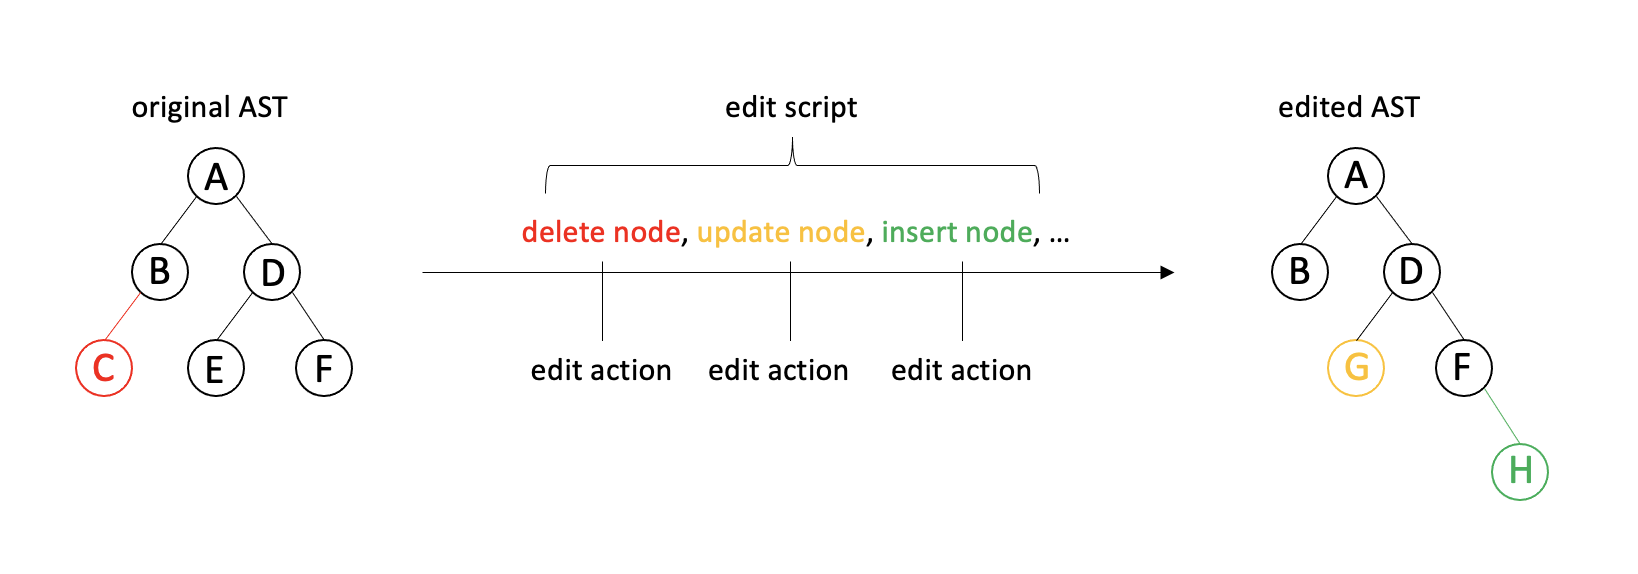
\includegraphics[width=\textwidth]{edit-action-script.png}
\end{figure}

\section{GumTree}

\textit{GumTree} is a source code differencing tool that has an AST-differencing algorithm at its core. It computes a short edit script between two input source files, and presents the changes close to programmers' intents in multiple formats~\cite{DBLP:conf/kbse/FalleriMBMM14}. In this project, I depend on the AST and edit script produced by GumTree to complete the refactoring detection.

\subsection{Edit Actions in GumTree}

GumTree defines 6 detectable types of edit actions to power its analysis.

\begin{enumerate}
	\item \textbf{Insert} Inserting a single node into the AST.
	\item \textbf{Delete} Removing a single node from the AST.
	\item \textbf{TreeInsert} Inserting a subtree into the AST.
	\item \textbf{TreeDelete} Removing a subtree from the AST.
	\item \textbf{Move} Relocating a subtree to a different position of the AST.
	\item \textbf{Update} Replacing a single node with another one.
\end{enumerate}
